\section{Elektromagnit induksiya qonuni.  Lens qoidasi.}





\begin{enumerate}

\item Faradeyning elektromagnit induksiya qonunining matematik ifodasini toping.
\begin{enumerate}[label=\Alph*)]
\item $\varepsilon=-kF/I$.
\item $\varepsilon=\dfrac{\Delta \Phi}{\Delta t}$.
\item $\varepsilon=-\dfrac{\Delta \Phi}{\Delta t}$.
\item $\varepsilon=k\dfrac{\Delta I}{\Delta \Phi \Delta t}$.
\item $\varepsilon=\dfrac{4\pi\varepsilon_0}{\Delta t}$.
\end{enumerate}

\item Induksiya EYK ning birligini ko‘rsating.
\begin{enumerate}[label=\Alph*)]
\item T/s.
\item B$\cdot$s.
\item Wb/s.
\item T$\cdot$m$^2$.
\item Wb$\cdot$s.
\end{enumerate}

\item Kuchlanish birligi Voltning o‘rniga yana qaysi birlikni ishlatsa bo‘ladi?
\begin{enumerate}[label=\Alph*)]
\item H/s.
\item Wb.
\item Wb/s.
\item H$\cdot$s.
\item Wb$\cdot$s.
\end{enumerate}

\item Berk kontur bir jinsli magnit maydonda induksiya chiziqlari bo‘ylab tezlanish bilan ilgarilanma harakat qilsa, induksiya EYK hosil bo‘ladimi?
\begin{enumerate}[label=\Alph*)]
\item bo‘ladi.
\item bo‘lmaydi.
\item bo‘ladi va chiziqli ravishda kamayib boradi.
\item bo‘ladi va chiziqli ravishda ortib boradi.
\item bo‘ladi va eksponensial ravishda o‘zgaradi.
\end{enumerate}

\item Konturda hosil bo‘luvchi induksiya EYK $50$ V bo‘lishi uchun konturni kesib o‘tuvchi magnit oqimning o‘zgarish tezligi qanday (Wb/s) bo‘lishi kerak?
\begin{enumerate}[label=\Alph*)]
\item 5.
\item 10.
\item 50.
\item 100.
\item 500.
\end{enumerate}

\item Kontur kesib o‘tuvchi magnit oqim $2$ s da $10$ Wb dan $2$ Wb gacha tekis kamaydi. Konturda hosil bo‘lgan induksiya EYK ni toping (V).
\begin{enumerate}[label=\Alph*)]
\item 10.
\item 8.
\item 4.
\item 2.
\item 0.
\end{enumerate}

\item Konturdan o‘tayotgan magnit oqim $0,3$ s davomida $9$ Wb dan $6$ Wb gacha tekis kamaygan bo‘lsa, konturda hosil bo‘lgan induksiya EYK necha Voltga teng?
\begin{enumerate}[label=\Alph*)]
\item 0,01.
\item 0,9.
\item 4,5.
\item 10.
\item 50.
\end{enumerate}

\item Berk kontur kesib o‘tuvchi magnit oqim $0,4$ s davomida $4\cdot10^{-5}$ Wb ga o‘zgardi. Induksiya EYK ni (V) aniqlang.
\begin{enumerate}[label=\Alph*)]
\item $4\cdot10^{-4}$.
\item $10^{-5}$.
\item $10^{-4}$.
\item $4\cdot10^{-5}$.
\item $2\cdot10^{-4}$.
\end{enumerate}

\item Solenoiddagi o‘ramlar soni $2,5$ marta ortsa, undagi induksiya EYK qanday o‘zgaradi?
\begin{enumerate}[label=\Alph*)]
\item o‘zgarmaydi.
\item 5 marta ortadi.
\item 5 marta kamayadi.
\item 2,5 marta ortadi.
\item 2,5 marta kamayadi.
\end{enumerate}

\item $200$ o‘ramga ega bo‘lgan g‘altak ichida magnit oqim $0,2$ s da $0,2$ Wb dan $1,1$ Wb gacha ortdi. G‘altakda induksiyalanadigan EYK ni aniqlang (V).
\begin{enumerate}[label=\Alph*)]
\item 1000.
\item 500.
\item 900.
\item 450.
\item 700.
\end{enumerate}

\item $100$ ta o‘ramdan iborat solenoiddagi magnit maydon oqimi $1$ ms davomida $5\cdot10^{-5}$ Wb dan $15\cdot10^{-5}$ Wb gacha o‘zgarsa, unda vujudga keluvchi induksion EYK necha Volt bo‘ladi?
\begin{enumerate}[label=\Alph*)]
\item 100.
\item 10.
\item 1.
\item 0,1.
\item 0,01.
\end{enumerate}

\item Magnit oqimning o‘zgarish tezligi $0,24$ Wb/s bo‘lganda, g‘altakda $48$ V elektr yurituvchi kuch hosil bo‘lsa, g‘altakdagi o‘ramlar soni qanday?
\begin{enumerate}[label=\Alph*)]
\item 200.
\item 250.
\item 260.
\item 300.
\item 20.
\end{enumerate}

\item Agar magnit oqimning o‘zgarish tezligi $60$ mWb/s bo‘lganda g‘altakda uyg‘onuvchi EYK $\varepsilon=12$ V bo‘lsa, g‘altakdagi o‘ramlar soni qanday?
\begin{enumerate}[label=\Alph*)]
\item 2000.
\item 3000.
\item 2500.
\item 300.
\item 200.
\end{enumerate}

\item Solenoiddagi magnit oqim $2$ ms da $3$ mWb dan $9$ mWb gacha o‘zgargan. Agar solenoidda hosil bo‘lgan EYK $60$ V bo‘lsa, solenoiddagi o‘ramlar soni qanday?
\begin{enumerate}[label=\Alph*)]
\item 5.
\item 20.
\item 180.
\item 200.
\item 300.
\end{enumerate}

\item O‘ramlar soni $80$ ta bo‘lgan tokli g‘altakda induksiya EYK $60$ V bo‘lsa, magnit oqimining o‘zgarish tezligi qanday (Wb/s)?
\begin{enumerate}[label=\Alph*)]
\item 1,33.
\item 0,8.
\item 0,75.
\item 0,48.
\item 0,7.
\end{enumerate}

\item Yopiq konturni kesib o‘tuvchi magnit oqimi $0,1$ Wb dan $1$ Wb gacha tekis ortganda, konturda $2,5$ V induksiya EYK hosil bo‘lgan bo‘lsa, magnit oqimi o‘zgarish vaqtini aniqlang(s).
\begin{enumerate}[label=\Alph*)]
\item 0,36.
\item 0,27.
\item 0,39.
\item 0,48.
\item 0,12.
\end{enumerate}

\item Yuzasi $30$ cm$^2$ bo‘lgan qo‘zg‘almas o‘ram bir jinsli magnit maydonda induksiya chiziqlariga perpendikulyar joylashgan. Agar magnit induksiyasi $0,01$ s dan $0,2$ T dan $0,7$ T gacha tekis ortsa, o‘ramda qanday induksiya EYK paydo bo‘ladi?
\begin{enumerate}[label=\Alph*)]
\item 500.
\item 50.
\item 15.
\item 0,15.
\item 0,045.
\end{enumerate}

\item O‘tkazgich halqa orqali magnit oqim $3$ s davomida $0,144$ Wb ga o‘zgargan. O‘tkazgichning qarshiligi $0,24~\Omega$ bo‘lsa, induksiya toki necha Amper?
\begin{enumerate}[label=\Alph*)]
\item 1,25.
\item 0,6.
\item 0,24.
\item 0,2.
\item 2,2.
\end{enumerate}

\item Qarshiligi $0,01~\Omega$ bo‘lgan kontur orqali o‘tuvchi magnit oqimi $2$ s da $0,012$ Wb ga tekis o‘zgarganda konturda hosil bo‘ladigan tok kuchini toping (A).
\begin{enumerate}[label=\Alph*)]
\item 2,4.
\item 0,1.
\item 0,6.
\item 0,68.
\item 1,6.
\end{enumerate}

\item Qarshiligi $0,8~\Omega$ bo‘lgan simdan ramka yasalgan. Ramka orqali o‘tuvchi magnit oqimi $4$ s ichida $6$ Wb dan $-10$ Wb gacha tekis kamaydi. Ramkada vujudga kelgan tok kuchini (A) toping.
\begin{enumerate}[label=\Alph*)]
\item 0,5.
\item 5.
\item 20.
\item 2.
\item 1.
\end{enumerate}

\item $N=8$ ta o‘ramli g‘altakka tushayotgan magnit maydon induksiyasi $\Delta t=0,5$ s ichida $B_1=0,8$ T dan $B_2=0,2$ T ga qadar kamaydi. G‘altak o‘ramining radiusi $r=10$ cm ga teng. Shu oraliqda g‘altakka ulangan $R=10~\Omega$ qarshilikdan oqib o‘tgan induksion tokni aniqlang. ($r$ g‘altak simining qarshiligini e’tiborga olmang.) $\pi=3$.

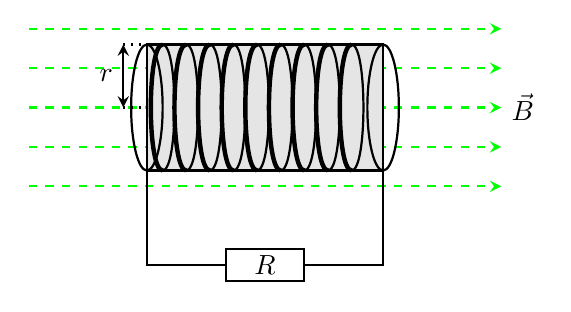
\begin{tikzpicture}[thick, scale=1]
    % Bir jinsli magnit maydon chiziqlari (B)
    \foreach \y in {0.5, 1, 1.5, 2, 2.5} {
        \draw[dashed, ->, >=stealth, green] (-1,\y) -- (5,\y);
    }
    \node[right] at (5, 1.5) {$\vec{B}$};

    % G'altakning asosi (silindr)
    \draw[fill=gray!20] (0.5, 0.7) rectangle (3.5, 2.3);
    \draw (0.5, 1.5) ellipse (0.2 and 0.8);
    \draw (3.5, 1.5) ellipse (0.2 and 0.8);
    
    % G'altak o'ramlari (solenoid spirali)
    \foreach \x in {0.7, 1.0, 1.3, 1.6, 1.9, 2.2, 2.5, 2.8, 3.1} {
        \draw (\x, 0.7) .. controls (\x+0.2, 0.7) and (\x+0.2, 2.3) .. (\x, 2.3);
        \draw[ultra thick] (\x, 2.3) .. controls (\x-0.2, 2.3) and (\x-0.2, 0.7) .. (\x, 0.7);
    }

    % Radius belgilash (r)
    \draw[<->, >=stealth] (0.2, 1.5) -- (0.2, 2.3);
    \node[left] at (0.2, 1.9) {$r$};
    \draw[dotted] (0.2, 1.5) -- (0.5, 1.5);
    \draw[dotted] (0.2, 2.3) -- (0.5, 2.3);

    % Tashqi zanjir va qarshilik (R)
    \draw (0.5, 0.7) -- (0.5, -0.5) -- (1.5, -0.5);
    \draw (3.5, 0.7) -- (3.5, -0.5) -- (2.5, -0.5);
    \draw (1.5, -0.7) rectangle (2.5, -0.3) node[midway] {$R$};

\end{tikzpicture}

\begin{enumerate}[label=\Alph*)]
\item 12,5.
\item 3,24.
\item 9,87.
\item 28,8.
\item 22,3.
\end{enumerate}

\item Induksiyasi $B$ bo‘lgan bir jinsli magnit maydonga o‘ramlari soni $N$ va kesim yuzasi $S$ bo‘lgan g‘altak joylashtiriladi. $t$ vaqt ichida 1-holatdan 2-holatga o‘tdi. Shu oraliqda g‘altakda hosil bo‘lgan induksiya EYK nimaga teng bo‘ladi?

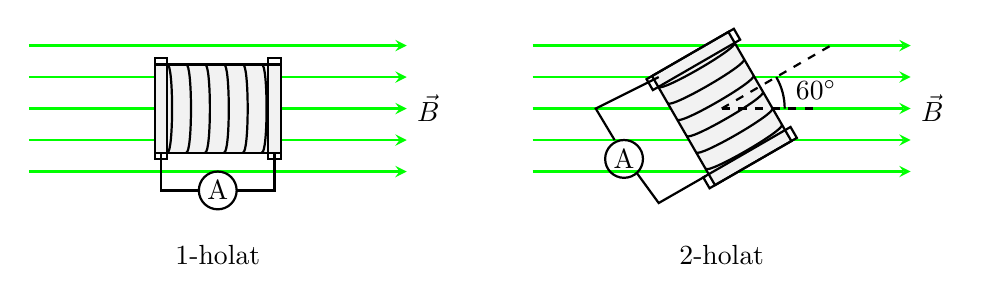
\begin{tikzpicture}[thick, scale=0.8]
    % --- 1-HOLAT ---
    \begin{scope}[xshift=0cm, ]
        % Magnit maydon chiziqlari (B)
        \foreach \y in {0.5, 1, 1.5, 2, 2.5} {
            \draw[->, >=stealth, green] (-1,\y) -- (5,\y);
        }
        \node[right] at (5, 1.5) {$\vec{B}$};

        % G'altak (Solenoid) - Gorizontal
        \draw[fill=gray!10] (1, 0.8) rectangle (3, 2.2);
        \draw (1, 0.7) rectangle (1.2, 2.3);
        \draw (2.8, 0.7) rectangle (3, 2.3);
        \foreach \x in {1.2, 1.5, 1.8, 2.1, 2.4, 2.7} {
            \draw (\x, 0.8) .. controls (\x+0.1, 0.8) and (\x+0.1, 2.2) .. (\x, 2.2);
        }

        % Ampermetrli zanjir
        \draw (1.1, 0.8) -- (1.1, 0.2) -- (1.7, 0.2);
        \draw (2.9, 0.8) -- (2.9, 0.2) -- (2.3, 0.2);
        \draw (2, 0.2) circle (0.3) node {A};
        
        \node[below] at (2, -0.5) {1-holat};
    \end{scope}

    % --- 2-HOLAT ---
    \begin{scope}[xshift=8cm]
        % Magnit maydon chiziqlari (B)
        \foreach \y in {0.5, 1, 1.5, 2, 2.5} {
            \draw[green,->, >=stealth] (-1,\y) -- (5,\y);
        }
        \node[right] at (5, 1.5) {$\vec{B}$};

        % Burilgan g'altak (60 gradus)
        \begin{scope}[rotate around={-60:(2,1.5)}]
            \draw[fill=gray!10] (1, 0.8) rectangle (3, 2.2);
            \draw (1, 0.7) rectangle (1.2, 2.3);
            \draw (2.8, 0.7) rectangle (3, 2.3);
            \foreach \x in {1.2, 1.5, 1.8, 2.1, 2.4, 2.7} {
                \draw (\x, 0.8) .. controls (\x+0.1, 0.8) and (\x+0.1, 2.2) .. (\x, 2.2);
            }
        \end{scope}

        % Burchakni belgilash
        \draw[dashed] (2,1.5) -- (3.5, 1.5);
        \draw[dashed] (2,1.5) -- +(30:2);
        \draw (3,1.5) arc (0:30:1);
        \node at (3.5, 1.8) {$60^\circ$};

        % Ampermetrli zanjir (burilgan holatda)
        \draw (1, 2) -- (0, 1.5) -- (0.3,1);
        \draw (1.75, 0.43) -- (1, 0) -- (0.65, 0.48);
        \draw (0.45, 0.7) circle (0.3) node {A};

        \node[below] at (2, -0.5) {2-holat};
    \end{scope}

\end{tikzpicture}

\begin{enumerate}[label=\Alph*)]
\item $-\dfrac{NBS}{t}$.
\item $-\dfrac{1}{2}\cdot\dfrac{NBS}{t}$.
\item $-\dfrac{\sqrt3}{2}\cdot\dfrac{NBS}{t}$.
\item $\dfrac{1}{2}\cdot\dfrac{NBS}{t}$.
\item $\dfrac{\sqrt3}{2}\cdot\dfrac{NBS}{t}$.
\end{enumerate}

\item Rasmda berk konturni kesib o‘tayotgan magnit oqimining vaqtga bog‘lanish grafigi keltirilgan. Qaysi oraliqda konturda hosil bo‘ladigan induksiya EYK nolga teng bo‘ladi(s)?

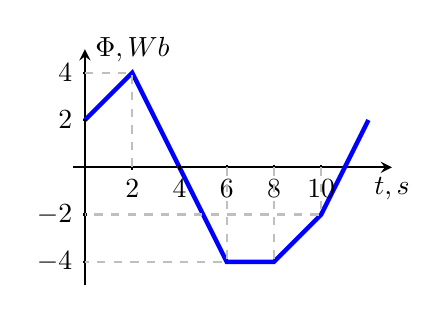
\begin{tikzpicture}[thick, scale=0.3, >=stealth]
    % Koordinata o'qlari
    \draw[->] (0,-5) -- (0,5) node[right] {$\Phi, \text{Wb}$};
    \draw[->] (-0.5,0) -- (13,0) node[below] {$t, \text{s}$};

    % Grafik chiziqlari (nuqtalar bo'yicha)
    \draw[blue, ultra thick] (0,2) -- (2,4) -- (6,-4) -- (8,-4) -- (10,-2)-- (12,2);

    % X-o'qidagi sonlar va yordamchi chiziqlar
    \foreach \x in {2, 4, 6, 8, 10} {
        \draw (\x, 0.1) -- (\x, -0.1) node[below] {$\x$};
    }

    % Y-o'qidagi sonlar va yordamchi chiziqlar
    \draw (0.1, 2) -- (-0.1, 2) node[left] {$2$};
    \draw (0.1, 4) -- (-0.1, 4) node[left] {$4$};
    \draw (0.1, -2) -- (-0.1, -2) node[left] {$-2$};
    \draw (0.1, -4) -- (-0.1, -4) node[left] {$-4$};

    % Punktir (yordamchi) chiziqlar
    \draw[dashed, gray!50] (0,4) -- (2,4) -- (2,0);
    \draw[dashed, gray!50] (6,0) -- (6,-4) -- (0,-4);
    \draw[dashed, gray!50] (8,0) -- (8,-4);
    \draw[dashed, gray!50] (10,0) -- (10,-2) -- (0,-2);

\end{tikzpicture}

\begin{enumerate}[label=\Alph*)]
\item 0$\div$2.
\item 2$\div$6.
\item 10$\div$12.
\item 8$\div$10.
\item 6$\div$8.
\end{enumerate}

\item Berk konturni kesib o‘tayotgan magnit oqimi vaqt bo‘yicha rasmda ko‘rsatilgandek o‘zgarsa, qaysi oraliqda konturda hosil bo‘ladigan induksiya EYK nolga bo‘ladi(s)?

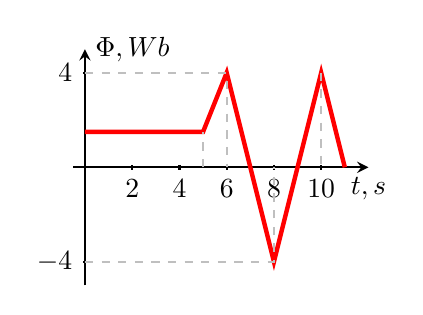
\begin{tikzpicture}[thick, scale=0.3, >=stealth]
    % Koordinata o'qlari
    \draw[->] (0,-5) -- (0,5) node[right] {$\Phi, \text{Wb}$};
    \draw[->] (-0.5,0) -- (12,0) node[below] {$t, \text{s}$};

    % Grafik chiziqlari (nuqtalar bo'yicha)
    % 0 dan 5 gacha o'zgarmas, keyin keskin tebranishlar
    \draw[red, ultra thick] (0,1.5) -- (5,1.5) -- (6,4) -- (8,-4) -- (10,4) -- (11,0);

    % X-o'qidagi sonlar va yordamchi chiziqlar
    \foreach \x in {2, 4, 6, 8, 10} {
        \draw (\x, 0.1) -- (\x, -0.1) node[below] {$\x$};
    }

    % Y-o'qidagi sonlar
    \draw (0.1, 4) -- (-0.1, 4) node[left] {$4$};
    \draw (0.1, -4) -- (-0.1, -4) node[left] {$-4$};

    % Punktir (yordamchi) chiziqlar
    \draw[dashed, gray!50] (5,0) -- (5,1.5);
    \draw[dashed, gray!50] (0,4) -- (6,4) -- (6,0);
    \draw[dashed, gray!50] (0,-4) -- (8,-4) -- (8,0);
    \draw[dashed, gray!50] (10,4) -- (10,0);

\end{tikzpicture}

\begin{enumerate}[label=\Alph*)]
\item 10$\div$12.
\item 5$\div$6.
\item 6$\div$8.
\item 8$\div$10.
\item 0$\div$5.
\end{enumerate}

\item Rasmda o‘ramni kesib o‘tayotgan magnit oqimning vaqtga bog‘lanish grafigi keltirilgan. O‘ramning qarshiligi $0,2~\Omega$ bo‘lsa, B--C oralig‘ida undagi tok kuchi qanday (mA)?

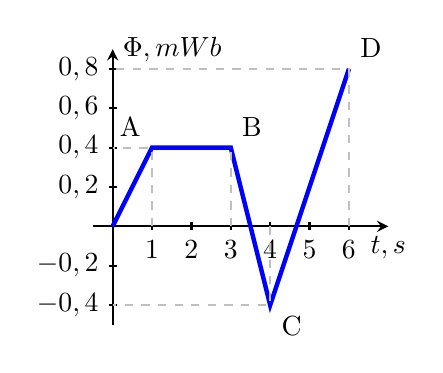
\begin{tikzpicture}[thick, scale=0.5, >=stealth]
    % Koordinata o'qlari
    \draw[->] (0,-2.5) -- (0,4.5) node[right] {$\Phi, \text{mWb}$};
    \draw[->] (-0.5,0) -- (7,0) node[below] {$t, \text{s}$};

    % Grafik chiziqlari (O-A-B-C-D nuqtalar bo'yicha)
    \draw[blue, ultra thick] (0,0) -- (1,2) node[above left, black] {A} 
    -- (3,2) node[above right, black] {B} 
    -- (4,-2) node[below right, black] {C} 
     -- (6,4) node[above right, black] {D};

    % X-o'qidagi sonlar va yordamchi chiziqlar
    \foreach \x in {1, 2, 3, 4, 5, 6} {
        \draw (\x, 0.1) -- (\x, -0.1) node[below] {$\x$};
    }

    % Y-o'qidagi sonlar (0.2 qadam bilan, lekin asosiy qiymatlar ko'rsatilgan)
    \draw (0.1, 1) -- (-0.1, 1) node[left] {$0,2$};
    \draw (0.1, 2) -- (-0.1, 2) node[left] {$0,4$};
    \draw (0.1, 3) -- (-0.1, 3) node[left] {$0,6$};
    \draw (0.1, 4) -- (-0.1, 4) node[left] {$0,8$};
    \draw (0.1, -1) -- (-0.1, -1) node[left] {$-0,2$};
    \draw (0.1, -2) -- (-0.1, -2) node[left] {$-0,4$};

    % Punktir (yordamchi) chiziqlar
    \draw[dashed, gray!50] (1,0) -- (1,2) -- (0,2);
    \draw[dashed, gray!50] (3,0) -- (3,2);
    \draw[dashed, gray!50] (4,0) -- (4,-2) -- (0,-2);
    \draw[dashed, gray!50] (6,0) -- (6,4) -- (0,4);

\end{tikzpicture}

\begin{enumerate}[label=\Alph*)]
\item 2.
\item 4.
\item 6.
\item 8.
\item 12.
\end{enumerate}

\item Qarshiligi $5~\Omega$ bo‘lgan o‘ramni kesib o‘tayotgan magnit oqim vaqt bo‘yicha rasmda ko‘rsatilgandek o‘zgarsa, o‘ramdagi tok kuchi $2$--$4$ s vaqt oralig‘ida necha Amper bo‘ladi?

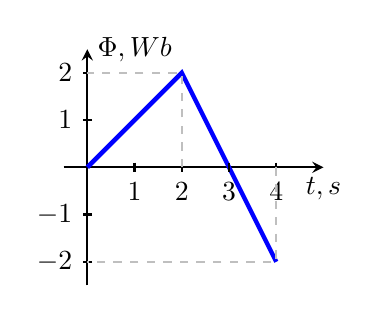
\begin{tikzpicture}[thick, scale=0.6, >=stealth]
    % Koordinata o'qlari
    \draw[->] (0,-2.5) -- (0,2.5) node[right] {$\Phi, \text{Wb}$};
    \draw[->] (-0.5,0) -- (5,0) node[below] {$t, \text{s}$};

    % Grafik chizig'i (nuqtalar: 0,0 -> 2,2 -> 4,-2)
    \draw[blue, ultra thick] (0,0) -- (2,2) -- (4,-2);

    % X-o'qidagi sonlar va yordamchi chiziqlar
    \foreach \x in {1, 2, 3, 4} {
        \draw (\x, 0.1) -- (\x, -0.1) node[below] {$\x$};
    }

    % Y-o'qidagi sonlar
    \draw (0.1, 1) -- (-0.1, 1) node[left] {$1$};
    \draw (0.1, 2) -- (-0.1, 2) node[left] {$2$};
    \draw (0.1, -1) -- (-0.1, -1) node[left] {$-1$};
    \draw (0.1, -2) -- (-0.1, -2) node[left] {$-2$};

    % Punktir (yordamchi) chiziqlar
    \draw[dashed, gray!50] (2,0) -- (2,2) -- (0,2);
    \draw[dashed, gray!50] (4,0) -- (4,-2) -- (0,-2);

\end{tikzpicture}

\begin{enumerate}[label=\Alph*)]
\item 2.
\item 0,4.
\item 0,2.
\item 0,1.
\item 0.
\end{enumerate}

\item Kvadrat shaklidagi ramka doimiy tezlik bilan harakatlanib bir jinsli magnit maydoni bo‘lgan sohadan o‘tadi (rasmga q.). Qaysi grafik ramkada hosil bo‘ladigan EYK ning vaqtga bog‘lanishini ifodalaydi?

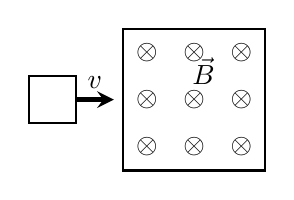
\begin{tikzpicture}[thick, scale=0.6]
    % Magnit maydoni sohasi (katta kvadrat)
    \draw (2,0) rectangle (5,3);
    
    % Magnit induksiya chiziqlari (o'quvchidan qog'oz ichiga yo'nalgan - X)
    \foreach \x in {2.5, 3.5, 4.5} {
        \foreach \y in {0.5, 1.5, 2.5} {
            \node at (\x,\y) {$\otimes$};
        }
    }
    \node[above] at (3.7, 1.6) {$\vec{B}$};

    % Kvadrat ramka (chapda, maydonga kirish arafasida)
    \draw (0,1) rectangle (1,2);
    
    % Tezlik vektori
    \draw[->, >=stealth, ultra thick] (1, 1.5) -- (1.8, 1.5) node[midway, above] {$v$};

\end{tikzpicture}

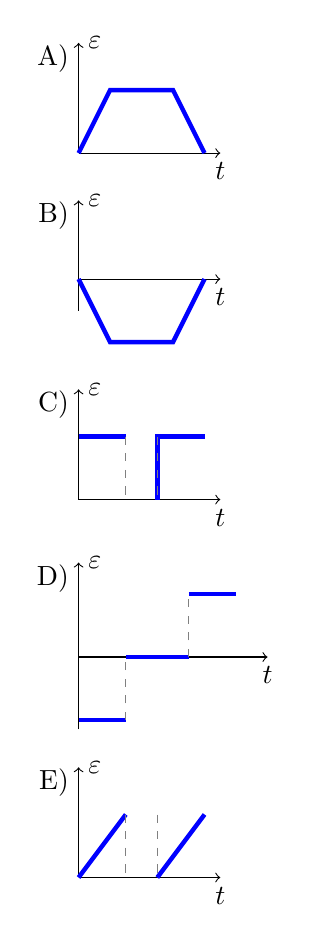
\begin{tikzpicture}[scale=0.4]

    % A variant
    \begin{scope}[xshift=0cm, yshift=0cm]
        \draw[->] (0,0) -- (0,3.5) node[right] {$\varepsilon$};
        \draw[->] (0,0) -- (4.5,0) node[below] {$t$};
        \draw[blue, ultra thick] (0,0) -- (1,2) -- (3,2) -- (4,0);
        \node[left] at (0,3) {A)};
    \end{scope}

    % B variant
    \begin{scope}[yshift=-4cm]
        \draw[->] (0,-1) -- (0,2.5) node[right] {$\varepsilon$};
        \draw[->] (0,0) -- (4.5,0) node[below] {$t$};
        \draw[blue, ultra thick] (0,0) -- (1,-2) -- (3,-2) -- (4,0);
        \node[left] at (0,2) {B)};
    \end{scope}

    % C variant
    \begin{scope}[yshift=-11cm]
        \draw[->] (0,0) -- (0,3.5) node[right] {$\varepsilon$};
        \draw[->] (0,0) -- (4.5,0) node[below] {$t$};
        \draw[blue, ultra thick] (0,2) -- (1.5,2) (1.5,0);
        \draw[blue, ultra thick] (2.5,0) -- (2.5,2) -- (4,2);
        \draw[dashed, gray] (1.5,2) -- (1.5,0) (2.5,2) -- (2.5,0);
        \node[left] at (0,3) {C)};
    \end{scope}

    % D variant (TO'G'RI JAVOB)
    \begin{scope}[yshift=-16cm]
        \draw[->] (0,-2.3) -- (0,3) node[right] {$\varepsilon$};
        \draw[->] (0,0) -- (6,0) node[below] {$t$};
        % Kirish (manfiy)
        \draw[blue, ultra thick] (0,-2) -- (1.5,-2);
        \draw[dashed, gray] (1.5,-2) -- (1.5,0);
        % Maydon ichida (nol)
        \draw[blue, ultra thick] (1.5,0) -- (3.5,0);
        % Chiqish (musbat)
        \draw[dashed, gray] (3.5,0) -- (3.5,2);
        \draw[blue, ultra thick] (3.5,2) -- (5,2);
        \node[left] at (0,2.5) {D)};
    \end{scope}

    % E variant
    \begin{scope}[yshift=-23cm]
        \draw[->] (0,0) -- (0,3.5) node[right] {$\varepsilon$};
        \draw[->] (0,0) -- (4.5,0) node[below] {$t$};
        \draw[blue, ultra thick] (0,0) -- (1.5,2);
        \draw[blue, ultra thick] (2.5,0) -- (4,2);
        \draw[dashed, gray] (1.5,2) -- (1.5,0) (2.5,2) -- (2.5,0);
        \node[left] at (0,3) {E)};
    \end{scope}

\end{tikzpicture}


\item Rasmda g‘altakni kesib o‘tayotgan magnit oqimning vaqtga bog‘lanish grafigi tasvirlangan. Induksiya EYKining vaqtga bog‘lanish grafigi qaysi rasmda to‘g‘ri berilgan?

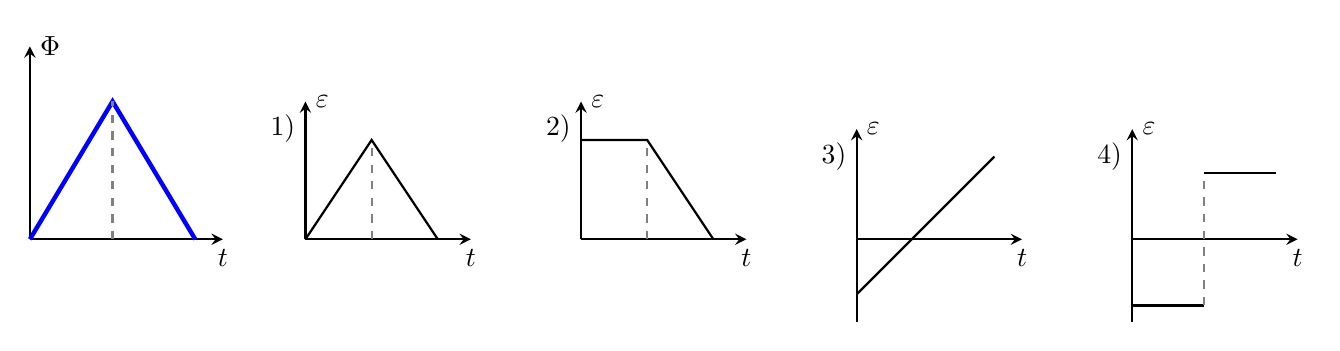
\begin{tikzpicture}[thick, scale=0.7, >=stealth]

    % --- ASOSIY GRAFIK: Magnit oqimi Phi(t) ---
    \begin{scope}[xshift=0cm, yshift=0cm]
        \draw[->] (0,0) -- (0,3.5) node[right] {$\Phi$};
        \draw[->] (0,0) -- (3.5,0) node[below] {$t$};
        \draw[blue, ultra thick] (0,0) -- (1.5,2.5) -- (3,0);
        \draw[dashed, gray] (1.5,0) -- (1.5,2.5);
        
    \end{scope}

    % --- 1-GRAFIK ---
    \begin{scope}[xshift=5cm, yshift=0cm]
        \draw[->] (0,0) -- (0,2.5) node[right] {$\varepsilon$};
        \draw[->] (0,0) -- (3,0) node[below] {$t$};
        \draw[black, thick] (0,0) -- (1.2,1.8) -- (2.4,0);
        \draw[dashed, gray] (1.2,0) -- (1.2,1.8);
        \node[left] at (0,2) {1)};
    \end{scope}

    % --- 2-GRAFIK ---
    \begin{scope}[xshift=10cm, yshift=0cm]
        \draw[->] (0,0) -- (0,2.5) node[right] {$\varepsilon$};
        \draw[->] (0,0) -- (3,0) node[below] {$t$};
        \draw[black, thick] (0,1.8) -- (1.2,1.8) -- (2.4,0);
        \draw[dashed, gray] (1.2,0) -- (1.2,1.8);
        \node[left] at (0,2) {2)};
    \end{scope}

    % --- 3-GRAFIK ---
    \begin{scope}[xshift=15cm, yshift=0cm]
        \draw[->] (0,-1.5) -- (0,2) node[right] {$\varepsilon$};
        \draw[->] (0,0) -- (3,0) node[below] {$t$};
        \draw[black, thick] (0,-1) -- (2.5,1.5);
        \node[left] at (0,1.5) {3)};
    \end{scope}

    % --- 4-GRAFIK (TO'G'RI JAVOB) ---
    \begin{scope}[xshift=20cm, yshift=0cm]
        \draw[->] (0,-1.5) -- (0,2) node[right] {$\varepsilon$};
        \draw[->] (0,0) -- (3,0) node[below] {$t$};
        % Phi ortganda epsilon manfiy o'zgarmas
        \draw[thick] (0,-1.2) -- (1.3,-1.2);
        \draw[dashed, gray] (1.3,-1.2) -- (1.3,1.2);
        % Phi kamayganda epsilon musbat o'zgarmas
        \draw[thick] (1.3,1.2) -- (2.6,1.2);
        \node[left] at (0,1.5) {4)};
    \end{scope}

\end{tikzpicture}

\begin{enumerate}[label=\Alph*)]
\item 4.
\item 3.
\item 2.
\item 1.
\item TJY.
\end{enumerate}

\item 1--5-rasmlarda kontur orqali magnit oqimning vaqtga bog‘lanish grafiklari tasvirlangan. Qaysi holda doimiy va musbat EYK hosil bo‘ladi?

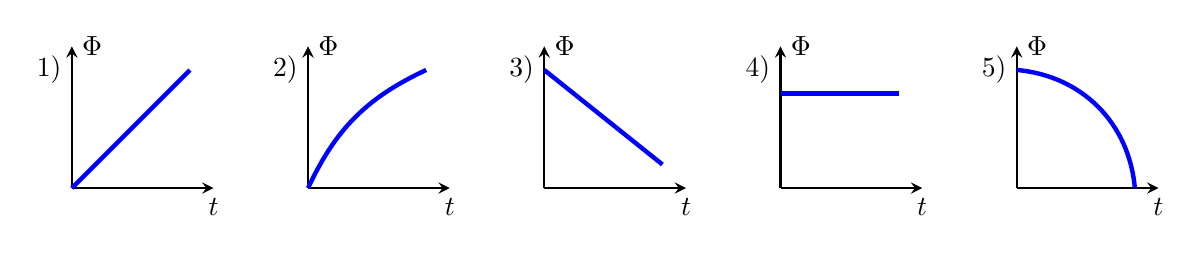
\begin{tikzpicture}[thick, scale=0.6, >=stealth]

    % 1-grafik (Chiziqli ortish)
    \begin{scope}[xshift=0cm, yshift=0cm]
        \draw[->] (0,0) -- (0,3) node[right] {$\Phi$};
        \draw[->] (0,0) -- (3,0) node[below] {$t$};
        \draw[blue, ultra thick] (0,0) -- (2.5,2.5);
        \node[left] at (0,2.5) {1)};
    \end{scope}

    % 2-grafik (Egri chiziqli ortish - parabola)
    \begin{scope}[xshift=5cm, yshift=0cm]
        \draw[->] (0,0) -- (0,3) node[right] {$\Phi$};
        \draw[->] (0,0) -- (3,0) node[below] {$t$};
        \draw[blue, ultra thick] (0,0) [bend right=-20] to (2.5,2.5);
        \node[left] at (0,2.5) {2)};
    \end{scope}

    % 3-grafik (Chiziqli kamayish - TO'G'RI JAVOB)
    \begin{scope}[xshift=10cm, yshift=0cm]
        \draw[->] (0,0) -- (0,3) node[right] {$\Phi$};
        \draw[->] (0,0) -- (3,0) node[below] {$t$};
        \draw[blue, ultra thick] (0,2.5) -- (2.5,0.5);
        \node[left] at (0,2.5) {3)};
    \end{scope}

    % 4-grafik (O'zgarmas oqim)
    \begin{scope}[xshift=15cm, yshift=0cm]
        \draw[->] (0,0) -- (0,3) node[right] {$\Phi$};
        \draw[->] (0,0) -- (3,0) node[below] {$t$};
        \draw[blue, ultra thick] (0,2) -- (2.5,2);
        \node[left] at (0,2.5) {4)};
    \end{scope}

    % 5-grafik (Egri chiziqli kamayish)
    \begin{scope}[xshift=20cm, yshift=0cm]
        \draw[->] (0,0) -- (0,3) node[right] {$\Phi$};
        \draw[->] (0,0) -- (3,0) node[below] {$t$};
        \draw[blue, ultra thick] (0,2.5) [bend left=40] to (2.5,0);
        \node[left] at (0,2.5) {5)};
    \end{scope}

\end{tikzpicture}

\begin{enumerate}[label=\Alph*)]
\item 1.
\item 2.
\item 3.
\item 4.
\item 5.
\end{enumerate}

\item Kontur orqali o‘tuvchi magnit oqimi $\Phi=-13,5t+0,28$ qonun bo‘yicha o‘zgarmoqda. Kontur qarshiligi $2,5~\Omega$ bo‘lsa, undagi induksion tokni aniqlang(A). [$\Phi$]=Veber.
\begin{enumerate}[label=\Alph*)]
\item 6,2.
\item 2,14.
\item 5,4.
\item 4,06.
\item 1,07.
\end{enumerate}

\item Qarshiligi $R=3,1~\Omega$ bo‘lgan kontur orqali o‘tuvchi magnit oqimi $\Phi=-5t^2-2t+5$ qonun bo‘yicha o‘zgarmoqda. Unda hosil bo‘lgan induksiya EYK ning va induksion tokning $t=6$ s vaqt momentidagi oniy qiymatini toping.
\begin{enumerate}[label=\Alph*)]
\item $\varepsilon_i=54$ V, $I_i=30$ A.
\item $\varepsilon_i=85$ V, $I_i=10$ A.
\item $\varepsilon_i=16$ V, $I_i=2$ A.
\item $\varepsilon_i=68$ V, $I_i=14$ A.
\item $\varepsilon_i=62$ V, $I_i=20$ A.
\end{enumerate}

\item O‘tkazgichdan yasalgan halqaning yuzi $25$ cm$^2$. Unga tik yo‘nalgan holda kesib o‘tuvchi magnit maydon induksiyasi $B=1,2+0,46t$ qonun bo‘yicha o‘zgaradi. Bu yerda [B]=Tesla, [t]=sekund. Halqada hosil bo‘lgan EYK qancha (mV) bo‘ladi?
\begin{enumerate}[label=\Alph*)]
\item 1,15.
\item 2,1.
\item 1.
\item 0,21.
\item 1,9.
\end{enumerate}

\item Qarshiligi $R=0,2~\Omega$, yuzasi $S=0,3$ m$^2$ bo‘lgan halqaga induksiyasi $B=2t-2,5t^2$ qonuni bo‘yicha o‘zgaruvchi magnit maydoni tushmoqda. Unda hosil bo‘lgan induksiya EYK ning va induksion tokning $t=4,4$ s vaqt momentidagi oniy qiymatini toping. [B]=Tesla.
\begin{enumerate}[label=\Alph*)]
\item $\varepsilon_i=86$ V, $I_i=2$ A.
\item $\varepsilon_i=67$ V, $I_i=1$ A.
\item $\varepsilon_i=56$ V, $I_i=5$ A.
\item $\varepsilon_i=6$ V, $I_i=30$ A.
\item $\varepsilon_i=15$ V, $I_i=75$ A.
\end{enumerate}

\item Qarshiligi $5~\Omega$ bo‘lgan o‘tkazgich halqani kesib o‘tuvchi magnit oqimi vaqt bo‘yicha rasmda ko‘rsatilgandek o‘zgarmoqda. Har uchala qismda hosil bo‘ladigan induksion toklarni aniqlang.

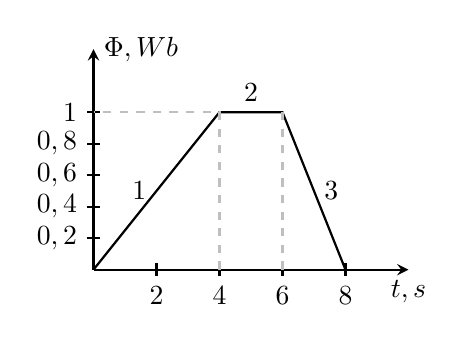
\begin{tikzpicture}[thick, scale=0.8, >=stealth]
    % Koordinata o'qlari
    \draw[->] (0,0) -- (0,3.5) node[right] {$\Phi, \text{Wb}$};
    \draw[->] (0,0) -- (5,0) node[below] {$t, \text{s}$};

    % Grafik chiziqlari (nuqtalar: 0,0 -> 2,2.5 -> 3,2.5 -> 4,0)
    % Masshtab: x-o'qi 1 birlik = 2s, y-o'qi 1 birlik = 0.4 Wb
    \draw[black, thick] (0,0) -- (2,2.5) node[midway, left] {1} 
    -- (3,2.5) node[midway, above] {2} 
    -- (4,0) node[midway, right] {3};

    % X-o'qidagi sonlar va yordamchi chiziqlar
    \foreach \x/\val in {1/2, 2/4, 3/6, 4/8} {
        \draw (\x, 0.1) -- (\x, -0.1) node[below] {$\val$};
    }

    % Y-o'qidagi sonlar
    \foreach \y/\val in {0.5/{0,2}, 1.0/{0,4}, 1.5/{0,6}, 2.0/{0,8}, 2.5/1} {
        \draw (0.1, \y) -- (-0.1, \y) node[left] {$\val$};
    }

    % Punktir (yordamchi) chiziqlar
    \draw[dashed, gray!50] (2,0) -- (2,2.5) -- (0,2.5);
    \draw[dashed, gray!50] (3,0) -- (3,2.5);

\end{tikzpicture}

\begin{enumerate}[label=\Alph*)]
\item 0,01 A; 0; 0,5 A.
\item 0,02 A; 0; 0,1 A.
\item 0,05 A; 0; 0,5 A.
\item 0,01 A; 0; 0,2 A.
\item 0,05 A; 0; 0,1 A.
\end{enumerate}

\item Qarshiligi $2~\Omega$ bo‘lgan konturni kesib o‘tuvchi magnit oqimi $0,1$ mWb dan $0,4$ mWb gacha tekis ortdi. O‘tkazgichning ko‘ndalang kesim yuzini vaqtda qancha o‘zgaradi (tadi)(mC)?
\begin{enumerate}[label=\Alph*)]
\item 0,2.
\item 0,4.
\item 0,15.
\item 0,12.
\item 0.
\end{enumerate}

\item Yuzi $200$ cm$^2$ bo‘lgan ramka induksiyasi $0,9$ T bo‘lgan bir jinsli magnit maydonda $50$ rad/s burchak tezlik bilan aylanmoqda. Ramkaning $40$ ta o‘ramida hosil bo‘ladigan EYK ning amplitudaviy qiymati necha Volt?
\begin{enumerate}[label=\Alph*)]
\item 36.
\item 40.
\item 16.
\item 25.
\item TJY.
\end{enumerate}

\item O‘ramlari soni $200$ ta va yuzi $150$ cm$^2$ bo‘lgan ramka induksiyasi $0,4$ T bo‘lgan bir jinsli magnit maydonda aylanmoqda. Ramkadagi EYK ning eng katta qiymati $6$ V bo‘lsa, ramka qanday burchak tezlik bilan aylanmoqda(rad/s)?
\begin{enumerate}[label=\Alph*)]
\item 30.
\item 3.
\item 5.
\item 23.
\item 16.
\end{enumerate}

\item Bir jinsli magnit maydonda aylantirilganda, ramkani kesib o‘tuvchi magnit oqim $\Phi=0,1\cos30t$ qonuni bo‘yicha o‘zgaradi. Ramkada hosil bo‘ladigan induksiya EYKning maksimal qiymati necha Voltga teng bo‘ladi? [$\Phi$]=Veber.
\begin{enumerate}[label=\Alph*)]
\item 30.
\item 3.
\item 1,5.
\item 0,3.
\item 0,1.
\end{enumerate}

\item Qarshiligi $R=20~\Omega$ bo‘lgan metall halqa bir jinsli magnit maydonda aylantirilganda, ramkani kesib o‘tuvchi magnit oqim $\Phi=8\cos1,5t$ qonuni bo‘yicha o‘zgaradi. Ramkada hosil bo‘ladigan induksiya EYK ning va induksion tokining $t=\pi/9$ s vaqt momentidagi oniy qiymatini toping. [$\Phi$]=Veber.
\begin{enumerate}[label=\Alph*)]
\item $\varepsilon_i=65$ V, $I_i=6$ A.
\item $\varepsilon_i=22$ V, $I_i=1,1$ A.
\item $\varepsilon_i=6$ V, $I_i=0,3$ A.
\item $\varepsilon_i=5$ V, $I_i=0,25$ A.
\item $\varepsilon_i=2$ V, $I_i=0,1$ A.
\end{enumerate}

\item O‘tkazgich rasmda ko‘rsatilgan magnit maydonda $v$ tezlik bilan harakatlanmoqda. Undagi induksion tok yo‘nalishini toping.

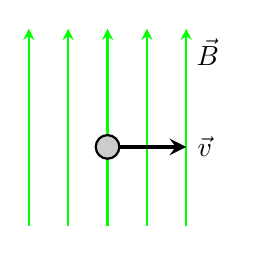
\begin{tikzpicture}[thick, scale=1]
    % Bir jinsli magnit maydon chiziqlari (B) - yuqoriga yo'nalgan
    \foreach \x in {0, 0.5, 1, 1.5, 2} {
        \draw[green, ->, >=stealth] (\x, 0) -- (\x, 2.5);
    }
    \node[right] at (2, 2.2) {$\vec{B}$};

    % O'tkazgich (doira shaklida kesimi tasvirlangan)
    \draw[fill=gray!40] (1, 1) circle (0.15);

    % Tezlik vektori (v) - o'ngga yo'nalgan
    \draw[->, >=stealth, ultra thick] (1.15, 1) -- (2, 1) node[right] {$\vec{v}$};

\end{tikzpicture}

\begin{enumerate}[label=\Alph*)]
\item o‘quvchiga qarab yo‘nalgan.
\item o‘tkazgichning harakat yo‘nalishida yo‘nalgan.
\item o‘quvchidan pastga qarab yo‘nalgan.
\item o‘tkazgichning harakatiga qarshi yo‘nalgan.
\item bu yerda induksion tok yuzaga kelmaydi.
\end{enumerate}

\item O‘tkazgich magnit qutblari orasida induksiya chiziqlariga tik bo‘lgan holda harakatlanmoqda. Undagi induksion tok o‘quvchi tomon yo‘nalgan bo‘lsa, o‘tkazgichning harakat yo‘nalishi qanday?

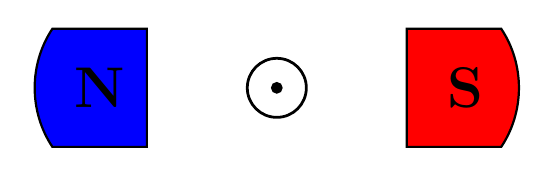
\begin{tikzpicture}[thick, scale=1.5]
    % Chap qutb (N - Shimol)
    \draw[fill=blue] (-1.2,0.5) -- (-2,0.5) .. controls (-2.2,0.8) and (-2.2,1.2) .. (-2,1.5) --(-1.2,1.5) -- cycle;
       
    \node[font=\huge\bfseries] at (-1.6, 1) {N};

    % O'ng qutb (S - Janub)
    \draw[fill=red, xshift=3cm] (-2, 0.5) -- (-1.2, 0.5) 
        .. controls (-1, 0.8) and (-1, 1.2) .. (-1.2, 1.5) 
        -- (-2, 1.5) -- cycle;
    \node[font=\huge\bfseries] at (1.5, 1) {S};

    % O'tkazgich (Markazda)
    \draw[fill=white, line width=1pt] (-0.1, 1) circle (0.25);
    \filldraw (-0.1, 1) circle (0.04); % Tok yo'nalishi: Nuqta (o'quvchiga qarab)
       

\end{tikzpicture}

\begin{enumerate}[label=\Alph*)]
\item chapga.
\item pastga.
\item o‘ngga.
\item tepaga.
\item TJY.
\end{enumerate}

\item Quyidagi rasmda to‘g‘ri o‘tkazgich ikkita magnit qutblari orasida harakatlanmoqda. Agar o‘tkazgichda induksion tok hosil bo‘lsa, magnit qutblarini aniqlang.

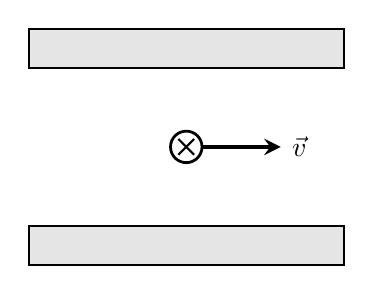
\begin{tikzpicture}[thick, scale=1]
    % Yuqorigi magnit qutbi
    \draw[fill=gray!20] (-2, 2.5) rectangle (2, 3);
    
    % Pastki magnit qutbi
    \draw[fill=gray!20] (-2, 0) rectangle (2, 0.5);

    % O'tkazgich (Markazda, ko'ndalang kesimi)
    \draw[fill=white, line width=1pt] (0, 1.5) circle (0.2);
    % Tok yo'nalishi: X (bizdan u tomonga/qog'oz ichiga)
    
    % Alternativ X chizish usuli:
    \draw[shift={(0,1.5)}] (-0.1,-0.1) -- (0.1,0.1);
    \draw[shift={(0,1.5)}] (-0.1,0.1) -- (0.1,-0.1);

    % Tezlik vektori (v) - o'ngga yo'nalgan
    \draw[->, >=stealth, ultra thick] (0.2, 1.5) -- (1.2, 1.5) node[right] {$\vec{v}$};

\end{tikzpicture}

\begin{enumerate}[label=\Alph*)]
\item yuqori-N; past-S.
\item yuqori-S; past-N.
\item yuqori-S; past-S.
\item yuqori-N; past-N.
\item ixtiyoriy bo‘lishi mumkin.
\end{enumerate}

\item Harakatlanayotgan o‘tkazgichda hosil bo‘ladigan induksiya EYK’i ifodasi qaysi javobda keltirilgan?
\begin{enumerate}[label=\Alph*)]
\item $\varepsilon=qvB\sin\alpha$.
\item $\varepsilon=vBl\sin\alpha$.
\item $\varepsilon=nevS$.
\item $\varepsilon=IBl\sin\alpha$.
\item $\varepsilon=-L\Delta I/\Delta t$.
\end{enumerate}

\item Uzunligi $0,7$ m bo‘lgan to‘g‘ri o‘tkazgich induksiyasi $5$ T bo‘lgan bir jinsli magnit maydonda $20$ m/s tezlik bilan harakatlanadi. Magnit induksiya vektori, tezlik vektori va o‘tkazgich o‘zaro perpendikular. O‘tkazgichda paydo bo‘ladigan induksiya EYK topilsin(V).
\begin{enumerate}[label=\Alph*)]
\item 60.
\item 70.
\item 80.
\item 90.
\item 100.
\end{enumerate}

\item $0,3$ m uzunlikka ega bo‘lgan o‘tkazgich $0,4$ T induksiyali bir jinsli magnit maydonda magnit induksiya vektoriga tik joylashgan. U o‘ziga tik yo‘nalishda magnit induksiya vektoriga $30^\circ$ burchak ostida $5$ m/s tezlik bilan harakatlanganda hosil bo‘ladigan induksiya EYK’i necha Voltga teng?
\begin{enumerate}[label=\Alph*)]
\item 0,1.
\item 0,2.
\item 0,3.
\item 0,5.
\item 0,8.
\end{enumerate}

\item $60$ cm uzunlikdagi o‘tkazgichni bir jinsli magnit maydonda induksiya chiziqlariga tik yo‘nalishda $5$ m/s tezlik bilan harakatlantirish natijasida $0,3$ V induksiya EYK hosil bo‘ldi. Magnit maydon induksiyasi qanday (T)?
\begin{enumerate}[label=\Alph*)]
\item 0,04.
\item 0,1.
\item 0,2.
\item 0,4.
\item 0,5.
\end{enumerate}

\item Uzunligi $0,4$ m bo‘lgan o‘tkazgich bir jinsli magnit maydon induksiya chiziqlariga va o‘ziga tik ravishda $5$ m/s tezlik bilan harakatlanganda, $0,6$ V induksiya EYK hosil bo‘lsa, magnit maydon induksiyasi necha Teslaga teng?
\begin{enumerate}[label=\Alph*)]
\item 0,3.
\item 0,4.
\item 0,5.
\item 0,2.
\item 0,6.
\end{enumerate}

\item Uzunligi $0,3$ m bo‘lgan to‘g‘ri o‘tkazgich magnit maydonini induksiya chiziqlariga $30^\circ$ burchak ostida $6$ m/s tezlik bilan kesib o‘tadi. Tezlik yo‘nalishi o‘tkazgichga tik. O‘tkazgichda induksiyalanuvchi EYK $3,6$ V ga teng bo‘lsa, maydonning magnit induksiyasi necha Tesla?
\begin{enumerate}[label=\Alph*)]
\item 1.
\item 2.
\item 3.
\item 4.
\item 6.
\end{enumerate}

\item Induksiyasi $0,5$ T bo‘lgan magnit maydonda induksiya chiziqlariga tik yo‘nalishda $6$ m/s tezlik bilan harakatlanayotgan o‘tkazgichda $12$ V EYK hosil bo‘lishi uchun uning uzunligi qanday bo‘lishi kerak(m)?
\begin{enumerate}[label=\Alph*)]
\item 1.
\item 2.
\item 3.
\item 4.
\item 6.
\end{enumerate}

\item Magnit induksiyasi $0,2$ T bo‘lgan maydonda aktiv qismining uzunligi $0,5$ m bo‘lgan o‘tkazgich induksiya chiziqlariga $30^\circ$ burchak ostida qanday tezlik bilan harakatlanganda, unda $0,8$ V induksiya EYK hosil bo‘ladi (m/s)?
\begin{enumerate}[label=\Alph*)]
\item 0,5.
\item 2.
\item 8.
\item 10.
\item 16.
\end{enumerate}

\item Induksiyasi $0,2$ T bo‘lgan bir jinsli magnit maydonda $20$ cm uzunlikdagi o‘tkazgichni induksiya chiziqlariga tik yo‘nalishda necha m/s tezlik bilan harakatlantirganda, unda $0,2$ V induksiya EYK hosil bo‘ladi?
\begin{enumerate}[label=\Alph*)]
\item 0,2.
\item 2.
\item 3.
\item 4.
\item 5.
\end{enumerate}

\item Induksiyasi $1$ T bo‘lgan magnit maydonda induksiya chiziqlariga tik yo‘nalishda harakatlanayotgan mis o‘tkazgichning $1$ A induksion tok hosil bo‘lishi uchun o‘tkazgichning tezligi necha m/s bo‘lishi kerak? O‘tkazgichning ko‘ndalang kesimi $0,017$ mm$^2$, misning solishtirma qarshiligi $1,7\cdot10^{-8}~\Omega\cdot$m.
\begin{enumerate}[label=\Alph*)]
\item 0,5.
\item 1.
\item 1,5.
\item 2.
\item 3.
\end{enumerate}

\item Yerning va bir-biridan izolyatsiyalangan temir yo‘l relslari millivoltmetr ulangan. Temir yo‘ldan $180$ km/h tezlik bilan poezd o‘tib ketayotganida, millivoltmetr nimani ko‘rsatadi (V)? Yer magnit maydonining induksiyasining vertikal tashkil etuvchisi $B=0,2\cdot10^{-4}$ T, relslar orasidagi masofa $1$ m.

\begin{enumerate}[label=\Alph*)]
\item 0.
\item $10^{-3}$.
\item $2\cdot10^{-3}$.
\item 20.
\item 220.
\end{enumerate}

\item Induksiyasi $15$ mT bo‘lgan magnit maydonda uzunligi $25$ cm, elektr qarshiligi $0,5~\Omega$ bo‘lgan sim doimiy $36$ km/h tezlik bilan rasmda ko‘rsatilgandek harakatlanmoqda. Konturda hosil bo‘lgan induksion tokni (mA) toping.

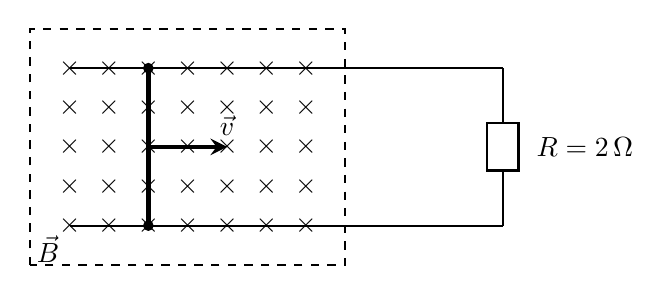
\begin{tikzpicture}[thick, scale=1]
    % Magnit maydoni sohasi (shtrixlangan kvadrat)
    \draw[dashed] (0,0) rectangle (4,3);
    
    % Magnit induksiya chiziqlari (bizdan qog'oz ichiga yo'nalgan - X)
    \foreach \x in {0.5,1, 1.5,2, 2.5,3, 3.5} {
        \foreach \y in {0.5,1, 1.5,2, 2.5} {
            \node at (\x,\y) {$\times$};
        }
    }
    \node[below left] at (0.5, 0.5) {$\vec{B}$};

    % Gorizontal relslar
    \draw (0.5, 2.5) -- (6, 2.5);
    \draw (0.5, 0.5) -- (6, 0.5);

    % Harakatlanuvchi vertikal o'tkazgich (stabel)
    \draw[ultra thick] (1.5, 0.5) -- (1.5, 2.5);
    \filldraw (1.5, 2.5) circle (1.5pt);
    \filldraw (1.5, 0.5) circle (1.5pt);

    % Tezlik vektori (v)
    \draw[->, >=stealth, ultra thick] (1.5, 1.5) -- (2.5, 1.5) node[above] {$\vec{v}$};

    % Rezistor (R)
    \draw (6, 2.5) -- (6, 1.8);
    \draw (6, 1.2) -- (6, 0.5);
    \draw (5.8, 1.2) rectangle (6.2, 1.8);
    \node[right] at (6.3, 1.5) {$R = 2 \, \Omega$};

\end{tikzpicture}

\begin{enumerate}[label=\Alph*)]
\item 20.
\item 30.
\item 15.
\item 75.
\item 50.
\end{enumerate}

\item Induksiyasi $4$ T bo‘lgan bir jinsli magnit maydonda induksiya chiziqlariga tik ravishda $5$ m/s tezlik bilan sim harakatlanmoqda. Bu sim uzunligi $20$ cm va qarshiligi $0,8~\Omega$ bo‘lsa, unda hosil bo‘lgan induksion tokni o‘lchovchi ampermetr nimani ko‘rsatadi? Bu tokning yo‘nalishini toping.

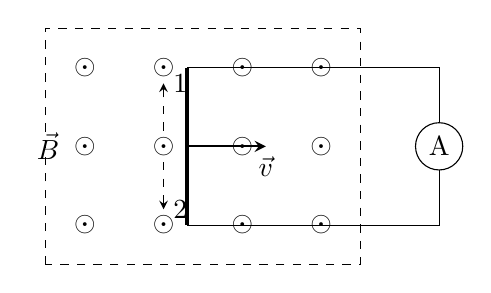
\begin{tikzpicture}
    % Magnit maydoni sohasi (shtrixlangan kvadrat)
    \draw[dashed] (0,0) rectangle (4,3);
    
    % Magnit induksiya chiziqlari (o'quvchi tomon yo'nalgan - nuqta)
    \foreach \x in {0.5, 1.5, 2.5, 3.5} {
        \foreach \y in {0.5, 1.5, 2.5} {
            \node at (\x,\y) {$\odot$};
        }
    }
    \node[left] at (0.3, 1.5) {$\vec{B}$};

    % Harakatlanuvchi o'tkazgich (stabel)
    \draw[fill=white, line width=1.5pt] (1.8, 0.5) -- (1.8, 2.5);
    
    % Tezlik vektori (v)
    \draw[->, >=stealth, thick] (1.8, 1.5) -- (2.8, 1.5) node[below] {$\vec{v}$};

    % Tok yo'nalishi belgilari (1 va 2)
    \draw[->, >=stealth, dashed] (1.5, 1.7) -- (1.5, 2.3) node[right] {1};
    \draw[->, >=stealth, dashed] (1.5, 1.3) -- (1.5, 0.7) node[right] {2};

    % Tashqi zanjir va Ampermetr
    \draw (1.8, 2.5) -- (5, 2.5) -- (5, 1.8);
    \draw (1.8, 0.5) -- (5, 0.5) -- (5, 1.2);
    \draw (5, 1.5) circle (0.3) node {A};

\end{tikzpicture}

\begin{enumerate}[label=\Alph*)]
\item 4 A, “1” yo‘nalishda.
\item 4 A, “2” yo‘nalishda.
\item 5 A, “1” yo‘nalishda.
\item 5 A, “2” yo‘nalishda.
\item 2 A, “1” yo‘nalishda.
\end{enumerate}

\item O‘tkazgichdan yasalgan halqa ichiga magnit janubiy qutbi bilan kiritila boshlaganda halqa magnitga tortiladimi, itariladimi?
\begin{enumerate}[label=\Alph*)]
\item itariladi.
\item tortiladi.
\item tortilmaydi ham, itarilmaydi ham.
\item tortilishi ham mumkin, itarilishi ham.
\item javob halqaning moddasiga bog‘liq.
\end{enumerate}

\item Magnit shimoliy qutbi bilan o‘tkazgich halqaga kiritilayotganda, halqa magnitga tortiladimi, itariladimi?
\begin{enumerate}[label=\Alph*)]
\item tortiladi.
\item itariladi.
\item tortilmaydi ham, itarilmaydi ham.
\item javob magnitning tezligiga bog‘liq.
\item javob halqaning diametriga bog‘liq.
\end{enumerate}

\item O‘tkazgichdan yasalgan halqa ipga osib qo‘yilgan. Unga o‘ramlaridan o‘zgaruvchan tok o‘tayotgan elektromagnit yaqinlashtirilsa, halqa qanday harakatlanadi?
\begin{enumerate}[label=\Alph*)]
\item elektromagnitga tortiladi.
\item elektromagnitdan itariladi.
\item gorizontal tebranadi.
\item vertikal tebranadi.
\item harakatlanmaydi.
\end{enumerate}

\item Doimiy magnit janubiy qutbi bilan metall halqadan uzoqlashtirilmoqda. Halqa magnitga tortiladimi yoki qochadimi? Halqaga magnit harakati yo‘nalishiga qaraganda induksion tok yo‘nalishi qanday bo‘ladi?

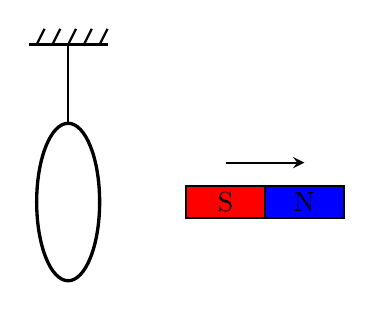
\begin{tikzpicture}[thick, scale=1]
    % Shift (shiftdagi osilgi nuqtasi)
    \draw (-0.5, 3) -- (0.5, 3);
    \foreach \x in {-0.4,-0.2,0,0.2,0.4}
        \draw (\x, 3) -- (\x+0.1, 3.2);

    % Ip va halqa
    \draw (0, 3) -- (0, 2);
    \draw[line width=1.2pt] (0, 1) ellipse (0.4 and 1);

    % Doimiy magnit (S va N qutblari bilan)
    % Magnit janubiy (S) qutbi bilan halqaga yaqin turibdi
    \draw[fill=red] (1.5, 0.8) rectangle (2.5, 1.2) node[midway] {S};
    \draw[fill=blue] (2.5, 0.8) rectangle (3.5, 1.2) node[midway] {N};

    % Harakat yo'nalishi (tezlik vektori)
    \draw[->, >=stealth, thick] (2, 1.5) -- (3, 1.5);

\end{tikzpicture}

\begin{enumerate}[label=\Alph*)]
\item tortiladi, soat strelkasi bo‘ylab.
\item tortiladi, soat strelkasiga qarama-qarshi.
\item qochadi, soat strelkasiga qarama-qarshi.
\item qochadi, soat strelkasi bo‘ylab.
\item tortiladi va tortilmaydi, tok kuchi nolga teng.
\end{enumerate}

\item Doimiy magnit shimoliy qutbi bilan metall halqaga yaqinlashtirilmoqda. Halqa magnitga tortiladimi yoki qochadimi? Halqaga magnit harakati yo‘nalishiga qaraganda induksion tok yo‘nalishi qanday bo‘ladi?

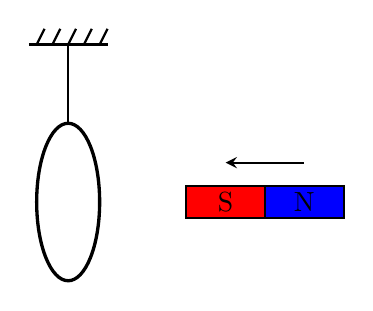
\begin{tikzpicture}[thick, scale=1]
    % Shift (shiftdagi osilgi nuqtasi)
    \draw (-0.5, 3) -- (0.5, 3);
    \foreach \x in {-0.4,-0.2,0,0.2,0.4}
        \draw (\x, 3) -- (\x+0.1, 3.2);

    % Ip va halqa
    \draw (0, 3) -- (0, 2);
    \draw[line width=1.2pt] (0, 1) ellipse (0.4 and 1);

    % Doimiy magnit (S va N qutblari bilan)
    % Magnit janubiy (S) qutbi bilan halqaga yaqin turibdi
    \draw[fill=red] (1.5, 0.8) rectangle (2.5, 1.2) node[midway] {S};
    \draw[fill=blue] (2.5, 0.8) rectangle (3.5, 1.2) node[midway] {N};

    % Harakat yo'nalishi (tezlik vektori)
    \draw[<-, >=stealth, thick] (2, 1.5) -- (3, 1.5);

\end{tikzpicture}

\begin{enumerate}[label=\Alph*)]
\item tortiladi, soat strelkasiga qarama-qarshi.
\item qochadi, soat strelkasi bo‘ylab.
\item qochadi, soat strelkasiga qarama-qarshi.
\item tortiladi, soat strelkasi bo‘ylab.
\item qochmaydi va tortilmaydi, tok kuchi nolga teng.
\end{enumerate}

\item Induksiyasi $B=8000(1+t^2)$ (T) qonun bo‘yicha o‘zgaruvchi magnit maydonda yuzi $50$ cm$^2$ bo‘lgan kvadrat ramka joylashgan. $t=1$ s vaqt momentida ramkada hosil bo‘lgan induksiya EYK nimaga teng? $(0-1)$ s oralig‘ida ramkaning K nuqtasida induksion tok qaysi yo‘nalishda o‘tadi?
\begin{enumerate}[label=\Alph*)]
\item 30 V; $(+)$ yo‘nalishda.
\item 40 V; $(-)$ yo‘nalishda.
\item 80 V; $(+)$ yo‘nalishda.
\item 30 V; $(-)$ yo‘nalishda.
\item 80 V; $(-)$ yo‘nalishda.
\end{enumerate}

\end{enumerate}

\begin{table}[!ht]
\centering
\begin{tabular}{|c|c|c|c|c|c|c|c|c|c|}
\hline
1c & 2c & 3b & 4b & 5c & 6c & 7d & 8c & 9d & 10c \\ \hline
11b & 12a & 13e & 14b & 15c & 16a & 17d & 18e & 19c & 20b \\ \hline
21d & 22d & 23e & 24e & 25b & 26b & 27d & 28a & 29c & 30c \\ \hline
31c & 32a & 33b & 34b & 35c & 36a & 37c & 38b & 39c & 40a \\ \hline
41e & 42a & 43b & 44b & 45c & 46a & 47d & 48d & 49d & 50e \\ \hline
51e & 52b & 53b & 54d & 55d & 56a & 57b & 58b & 59a & 60c \\ \hline
61e &  &  &  &  &  &  &  &  &  \\ \hline
\end{tabular}
\end{table}
